\def\thudbabelopt{english}
\documentclass[target=bach,aauheader=]{thud}

%% --- Information about the thesis --- %%
\course{Internet of Things, Big Data and Web}
\title{Comparison of tools for the formal verification of MTProto 2.0}
\author{Alessandro Zanatta}
\supervisor{Prof.\ Marino Miculan}
%% \cosupervisor{Prof.\ Nicola Vitacolonna} % TODO: Is Vitacolonna considered a supervisor?
%% Other available fields: \reviewer, \tutor, \chair, \date (anno accademico, calcolato in automatico), \rights

%% --- Suggested packages ---
%% pdfx: per generare il PDF/A per l'archiviazione. Necessario solo per la versione finale
\usepackage[a-1b]{pdfx}
%% hyperref: Regola le impostazioni della creazione del PDF... più tante altre cose. Ricordarsi di usare l'opzione pdfa.
\usepackage[pdfa]{hyperref}
%% tocbibind: Inserisce nell'indice anche la lista delle figure, la bibliografia, ecc.

%% --- Stili di pagina disponibili (comando \pagestyle) ---
%% sfbig (predefinito): Apertura delle parti e dei capitoli col numero grande; titoli delle parti e dei capitoli e intestazioni di pagina in sans serif.
%% big: Come "sfbig", solo serif.
%% plain: Apertura delle parti e dei capitoli tradizionali di LaTeX; intestazioni di pagina come "big".

%% --- Other packages --- %%
\usepackage{msc} % Protocol graphical representation
\usepackage{mathtools}
\usepackage{amssymb}
\usepackage{enumitem}
\usepackage[justification=centering]{caption} % Used to have always centered captions
\usepackage{cleveref} % better references
\usepackage{graphicx} % for images
\usepackage{textgreek} % greek letters out of math mode
\graphicspath{ {./images} } % images path

%% --- Commands --- %%
\newcommand\setmscoptions{%
  \setlength{\instdist}{5cm}%
  % \setlength{\levelheight}{1.5 \levelheight}%
  % \setlength{\instwidth}{3cm}
  \setmsckeyword{}
  \drawframe{no}
  \centering
}

% Multiline comments
\newcommand{\comment}[1]{}

\newcommand*{\Z}{\mathbb{Z}}
\newcommand*{\Q}{\mathbb{Q}}

%% Taken from https://hal.inria.fr/file/index/docid/955869/filename/sapic.tex
\newcommand{\msrewrite}[1]{\mathrel{-\hspace{-2pt}[#1]\hspace{-4pt}\to}}
\newcommand{\emptyrule}{\ensuremath{[]}\xspace}
\newcommand{\msr}[3]{\ensuremath{#1 \msrewrite{#2} #3}}
%% -------------- %%

\newcommand{\msrnolabel}[2]{\ensuremath{#1 \rightarrow #2}}
\newcommand{\msrsetminus}{\ensuremath{\setminus^\#}}
\newcommand{\msrcap}{\ensuremath{\cap^\#}}
\newcommand{\msrcup}{\ensuremath{\cup^\#}}
\newcommand{\msrin}{\ensuremath{\in^\#}}
\newcommand{\msrsubseteq}{\ensuremath{\subseteq^\#}}
\newcommand{\lin}[1]{\ensuremath{lin\left(#1\right)}}
\newcommand{\pers}[1]{\ensuremath{pers\left(#1\right)}}

\newcommand{\fact}[2]{\ensuremath{\mbox{!#1}\left(#2\right)}}
\newcommand*{\myexp}{\hat{\mkern6mu}}

%% --- Document start --- %%
\begin{document}
\maketitle

%% Dedica (opzionale)
\begin{dedication}
	Al mio cane,\par per avermi ascoltato mentre ripassavo le lezioni.
\end{dedication}

%% Ringraziamenti (opzionali)
\acknowledgements
Ringraziamenti vari qua

%% Sommario (opzionale)
\abstract
Un bell'abstract va qua!

%% Indice
\tableofcontents

%% Lista delle tabelle (se presenti)
%\listoftables

%% Lista delle figure (se presenti)
%\listoffigures

%% Corpo principale del documento
\mainmatter

%% Capitolo
\chapter{Introduction}


\chapter{Proverif and Tamarin-Prover}

We are going to discuss about two tools for cryptographic protocol verification: \href{https://prosecco.gforge.inria.fr/personal/bblanche/proverif/}{Proverif} and \href{https://tamarin-prover.github.io/}{Tamarin-Prover} . Tamarin-Prover will also be referred to as Tamarin for brevity.

First of all, let us consider the different types of approaches to security protocol analysis. The two categories of techniques are shown in figure \ref{fig:symbolic-computational-model} and we will proceed examining them.

\begin{figure}[!h]
    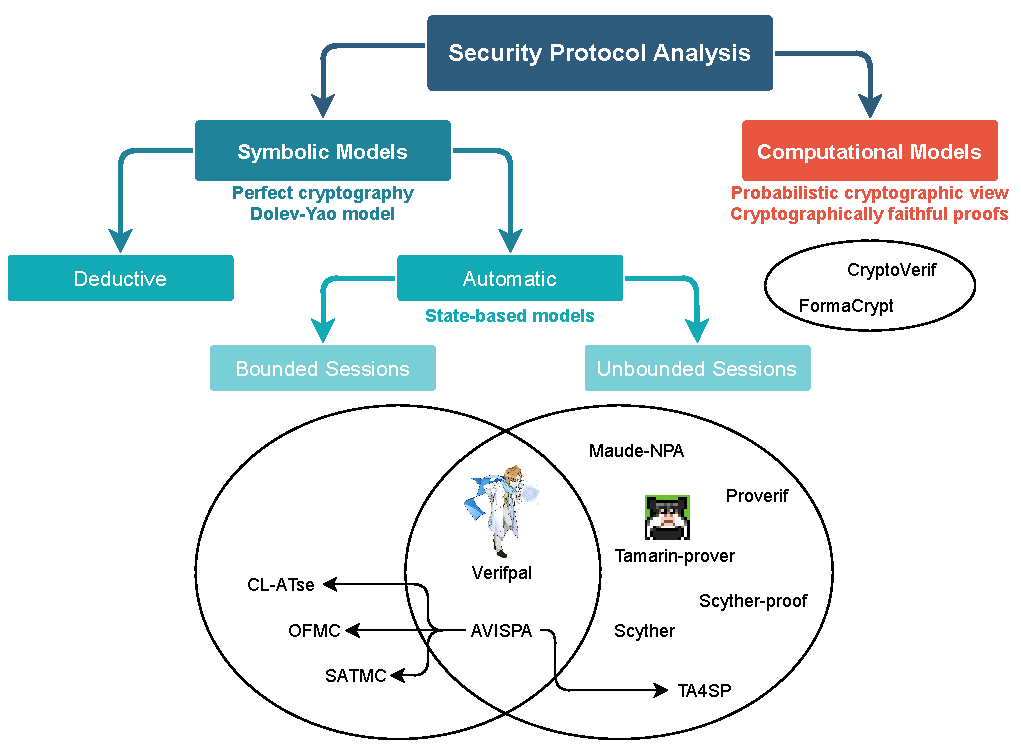
\includegraphics[scale=0.9]{symbolic-computational-model}
    \centering
    \label{fig:symbolic-computational-model}
    \caption{Symbolic and computational models}
\end{figure}

In the \textit{symbolic model} (often called Dolev-Yao model) \cite{Dolev-Yao}, the cryptographic primitives are considered as black-box and are represented using function symbols, the messages are terms and the adversary can only use defined primitives. An important aspect to note of this model is that it assumes \textbf{perfect cryptography}. As an example, consider the case in which there are two function symbols (\textbf{enc} and \textbf{dec}, used to encrypt and decrypt), a message \textit{m} and a key \textit{k} and the following equality is defined:

\begin{equation}
\mbox{dec}\left(\mbox{enc}\left(m, k\right), k\right) = m
\end{equation}

Following from the equation $-$ and considering the perfect cryptography assumption $-$ it is possible to decrypt $\mbox{enc}\left(m, k\right)$ if and only if \textit{k} is known \cite{SymbolicComputationalBlanchet}.


In the \textit{computational model} the messages are bitstrings, the cryptographic primitives are functions from bitstrings to bitstrings and the attacker is modeled as a probabilistic Turing machine.
A security property in this model is considered to hold when the probability that it does \textit{not} hold is negligible. For instance, the previously discussed shared-key encryption can be modeled using the same equalities, but the security of encryption is expressed by stating that the attacker has an insignificant probability of breaking the primitive (e.g. decrypting the message without having the key). Security proofs using this model are usually stronger, however this comes to the cost of long, difficult, tedious and highly error prone proofs (as stated by INRIA researchers \cite{ComputationalAnalysisCryptoSystemsINRIA}). Finally, as pointed to by Blanchet \cite{SymbolicComputationalBlanchet}, the computational model is indeed just a \textit{model} and ignores many aspects of reality and potential attacks, e.g. faulty attacks like the RSA one \cite{RSAFaultAttack}. 

Both Proverif and Tamarin employ a symbolic model. This makes it possible to automate proofs when given a set of primitives, a protocol model and a set of security properties. Note that termination is still not always guaranteed \footnote{It actually depends on the tool. Proverif proofs always terminate, but they might terminate with an inconclusive result, while Tamarin may simply not terminate without ever giving a result. More details about this problem will be discussed later.}. % TODO: discuss non termination issues!!

\section{Proverif}
% TODO

\section{Tamarin}
In this section we will see an overview of Tamarin foundations and internal reasoning.
For a more in-depth description and further information, see the Tamarin foundations paper \cite{TamarinFoundations} or the extended foundations paper \cite{TamarinFoundationsExtended}.

\subsection{High level view}
First of all, let's have a look at an high level picture of Tamarin.

The security property model of Tamarin is based on multiset rewriting rules to specify protocols and adversary capabilities, a guarded fragment \footnote{Only a few examples of formulas respecting the guarded fragment of first order logic used by Tamarin will be given in the next subsections. See \cite{FragmentFirstOrderLogicPaper} for a rigorous definition from a mathematical point of view.} of first order logic to specify security properties \footnote{Security properties in Tamarin will also be referred to as \textit{lemmas}.} and functions and equational theories to model the algebraic properties of cryptographic protocols \cite{TamarinFoundations}. % TODO: show a few examples of first order logic formulas respecting the guarded fragment!!

Given the rewriting rules, security properties and equational theories, Tamarin uses a novel constraint-solving algorithm which tries to validate or falsify lemmas.

Tamarin also offers builtin equational theories \cite{TamarinProverManual}. A brief overview will be given in subsection \ref{sub:Builtin-equational-theories}.

\subsection{Transition rules}
\label{sub:Transition-rules}
As reported earlier, multiset rewriting rules are used to specify adversary capabilities and protocols. More precisely, a \textit{set} of \textit{labeled} multiset rewriting rules are used.

The components for these multisets are the following:

\begin{description}[style=nextline]
    \item[Terms] which can be essentially thought of as messages. Terms can be of three different sorts. The more general sort is the \textit{msg} sort, which has two incomparable subsorts \textit{fresh} and \textit{pub} for fresh and public names;
    \item[Facts] which model information in the protocol. Facts have an arity, can be linear or persistent and are composed by terms. By convention, they always start with a capital letter;
    \item[Special facts] Four facts are reserved and are used to model the freshness of a message $t$ ($\mbox{\textbf{Fr}}\left(t\right)$), a message $t$ coming from the public channel ($\mbox{\textbf{In}}\left(t\right)$), a message $t$ to be output to the public channel ($\mbox{\textbf{Out}}\left(t\right)$) and knowledge of a certain message $t$ from the attacker ($\mbox{\textbf{K}}\left(t\right)$);
    \item[State of the system] The state of the system is represented using a finite \textit{multiset} of facts;
    \item[Transition rules] A multiset of transition rules defines the possible transitions from one state to another one. Transitions are denoted with the following syntax
    \begin{equation}
        L \msrewrite{A} R
    \end{equation}
    where $L, A$ and $R$ are multisets of facts.
\end{description}

Let us examine an informal description of transitions.

\begin{itemize}
    \item{Let $S$ be the current state of the system}
    \item{Let $\msrnolabel{L}{R}$ be a transition rule. Note that this is a \textit{multiset rewriting rule} without a \textit{label};}
    \item{Let $\msrnolabel{l}{r}$ be a ground instance of the rule (i.e. no variables are present in the multisets);}
    \item{If we apply $\msrnolabel{l}{r}$ to our state $S$ we reach a new state, defined by the following equation:
    \begin{equation}
        S \msrsetminus l \msrcup r
    \end{equation}
    We use $\msrsetminus$ and $\msrcup$ to define difference and union over multisets, respectively;}
    \item{When we use labelled multiset rewriting rules, such as $\msr{l}{a}{r}$, we also add facts from $a$ to the \textit{trace} of the execution.}
\end{itemize}

Tamarin defines two transition rules


\subsection{Builtin equational theories}
\label{sub:Builtin-equational-theories}
A brief list of Tamarin built-ins is given below: \footnote{Only the builtin theories considered relevant and those used in the analysis will be described here. The full list is available in the Tamarin manual. \cite{TamarinProverManual}}

\begin{description}[style=nextline]
    \item[hashing] defines a perfect hash function \textbf{h/1} \footnote{The writing \textbf{f/x} indicates that the function \textbf{f} has arity \textbf{x}.};
    \item[asymmetric-encryption] models a public key encryption scheme. It defines the following symbols:
    
    \begin{itemize}
        \item{\textbf{aenc/2}, used to model the encryption of a message with a public key}
        \item{\textbf{adec/2}, used to model the decryption of an encrypted message with a private key}
        \item{\textbf{pk/1}, used to derive a public key from a private key}
    \end{itemize}

    Functions are related by the equation \textbf{adec(aenc(msg, pk(sk)), sk) = msg};

    \item[diffie-hellman] models Diffie-Hellman groups. It defines the following symbols:
    
    \begin{itemize}
        \item{\textbf{inv/1}, models the inverse of an element}
        \item{\textbf{1/0}, models the neutral element}
        \item{\textbf{\textasciicircum} and \textbf{*} symbols, models exponentiation and multiplication respectively}
    \end{itemize}

    The equational theory for this builtin is actually quite complex. For the sake of completeness, these are the related equations:
    \begin{itemize}
        \item{(x \textasciicircum y) \textasciicircum z = x \textasciicircum (y * z)}
        \item{x \textasciicircum 1 = x}
        \item{x * y = y * x}
        \item{(x * y) * z = x * (y * z)}
        \item{x * 1 = x}
        \item{x * inv(x) = 1}
    \end{itemize}
    % TODO: parla ancora un po' di quanto sia figo Tamarin che ha DH builtin!
\end{description}

\section{Comparison of Proverif and Tamarin}

\chapter{MTProto2.0 protocol description}

In this chapter, we will give a brief overview of the MTProto2.0 protocol. A more in-depth and formal description can be found on the official web page \cite{Telegram-MTProto2.0}.

First of all, MTProto2.0 is a \textit{suite of protocols} used to enable secure communication between a Telegram client and a Telegram server over an insecure network. MTProto2.0 can be decomposed in the three following protocols:

\begin{description}[style=nextline]
    \item[Authorization] used to obtain a secret authorization key shared only with the server;
    \item[Secret-chat] used to obtain a secret key shared between two clients. This is then used to exchange end-to-end messages between two clients, with the server that basically acts as a forwarder;
    \item[Rekeying] used to achieve Perfect Forward Secrecy, allows obtaining a new end-to-end encryption key.
\end{description}

Additionally, the cloud chats encryption schema is used to securely exchange messages between clients and servers (who have shared an authorization key).

An overview on these protocols will be given in \cref{sec:auth-prot,sec:cloud-chat,sec:secret-chat,sec:rekeying}.

\section{Authorization protocol}
\label{sec:auth-prot}

%% Authorization protocol %%
\begin{figure}[!t]
\setlength{\instdist}{4cm}
\setmscoptions
\begin{msc}{}
\setmscscale{.8} 

\declinst{client}{}{Client}
\declinst{server}{}{Server}

\action*{Generates nonces $n_{c}, n_{k}$}{client}
\action*{\parbox{4.5cm}{\centering 
    Knows keys $\mbox{sk}^{(1)}, \dots, \mbox{sk}^{(n)}$\\
    Generates $n_s, g, p$\\
    Generates proof-of-work primes $q, r$
}}{server}
\nextlevel[6]

\mess{$n_{c}$}{client}{server}
\nextlevel[2]
\mess{$n_{c}, n_{s}, q \cdot r, \mbox{fp}^{(1)}, \dots, \mbox{fp}^{(n)}$}{server}{client}

\nextlevel
\action*{\parbox{4cm}{\centering
    Chooses $\mbox{pk}^{(i)}$ matching\\
    $\mbox{fp}^{(i)}$ for some $i$\\
    Factorizes $q \cdot r$\\
    $C_1 := q \cdot r, q, r, n_c, n_s, n_k$
}}{client}

\nextlevel[7]
\mess{$n_c, n_s, q, r, \mbox{fp}^{(i)}, \{\mbox{sha1}\left(C_1\right), C_1\}_{\mbox{pk}^{(i)}}$}{client}{server}
\nextlevel

\action*{$\left(k, iv\right) := \mbox{kdf}\left(n_s, n_k\right)$}{client}
\action*{\parbox{4.5cm}{\centering
    $s \in \Z_p$\\
    $g_s := g^s \mod{p}$\\
    $key, iv := \mbox{kdf}\left(n_s, n_k\right)$\\
    $S_1 := n_c, n_s, g, p, g_s, t_1$
}}{server}

\nextlevel[6]
\mess{$n_c, n_s, \left\{\mbox{sha1}\left(S_1\right), S_1\right\}_{key, iv}$}{server}{client}
\nextlevel

\action*{\parbox{4.5cm}{\centering
$c \in \Z_p$\\
$g_c := g^c \mod{p}$\\
Checks $g, p$\\
$k_{CS} := g_s^c \mod{p}$\\
$C_2 := n_c, n_s, rID, g_c$
}}{client}
\nextlevel[7]

\mess{$n_c, n_s, \left\{\mbox{sha1}\left(C_2\right), C_2\right\}_{k, iv}$}{client}{server}
\nextlevel

\action*{\parbox{4.5cm}{\centering
$k_{CS} := g_c^s \mod{p}$
}}{server}
\nextlevel[3]

\mess{$n_c, n_s, \mbox{hash}\left(n_k, k_{CS}\right)$}{server}{client}


\end{msc}
\centering
\caption{MTProto2.0 Authorization protocol}
\label{fig:authorization-protocol}
\end{figure}


The first time a Telegram client C runs the application, it must negotiate an \textbf{authorization key} with the Telegram server S. The authorization protocol is used to this end. Once the client and the server have shared an authorization key, they will use it to encrypt (almost) every future communication between them. A client might also have several keys (e.g. on multiple devices or if reinstalling the application), some of which might be locked (e.g. if the device is lost). The authorization protocol is based on the Diffie-Hellman key exchange protocol \cite{DH-protocol}.


A successful protocol run consists of three rounds, which are represented schematically in \cref{fig:authorization-protocol}:
\begin{description}
    \item[Round 1] In the first round messages are in plaintext. In particular, the client and the server exchange two nonces ($n_c$ and $n_s$). The pair $\left<n_c, n_s\right>$ identifies a session of the authorization protocol. These nonces are sent in every consequent message of the current run of the protocol, both in plaintext and encrypted form.
    \begin{enumerate}
        \item{In the first message, the client sends his fresh nonce $n_c$ to the server;}
        \item{The server answers with the client nonce $n_c$, the server fresh nonce $n_s$, a challenge $q \cdot r \leq 2^{63}$ (which are two primes used as a measure to prevent denial of service, as the client needs to spend resources on factorizing $q \cdot r$ before the server has to commit (more) resources\footnote{Notice that this might not be true as this is vulnerable to a lookup table approach (e.g. using \href{http://factordb.com}{factordb.com}).}) and a list of public RSA key fingerprints (calculated as the lower 64-bits of the SHA1 of the server public keys).}
    \end{enumerate}

    \item[Round 2] The client decomposes $q\cdot r$ in $\left<q, r\right>$, retrieves the public key of the server $pk^{\left(i\right)}$. The client then generates a nonce $n_k$ of 256 bits. This nonce $n_k$ is supposed to be secret. The pair $\left<n_s, n_k\right>$ is used, by both server and client, to derive, through a derivation function $\mbox{kdf}$, a symmetric encryption key $k$ and an initialization vector $iv$, which will be used in subsequent exchanges.
    \begin{enumerate}
        \setcounter{enumi}{2}
        \item{The client asymmetrically encrypts both $\left<q\cdot r, q, r, n_c, n_s, n_k\right>$ and its SHA1 hash with $pk^{(i)}$ and sends it along with $\left<n_c, n_s, q, r, fp^{(i)}\right>$ to the server. A rather complex padding schema is used;}
        \item{The server generates his Diffie-Hellman ephemeral key $s$ of 2048-bits, chooses $g, p$ and computes $g_s = g^s \mod{p}$. Finally, it symmetrically encrypts both $\left<n_c, n_s, g, p, g_s, t_1\right>$ and its SHA1 hash and sends it along with $\left<n_c, n_s\right>$.}
    \end{enumerate}

    Notice that the client is supposed to check that:
    \begin{itemize}
        \item{$p$ is a safe 2048-bit prime, where safe means that both $p$ and $\frac{p-1}{2}$ are prime and $2^{2047} < p < 2^{2048}$;}
        \item{$g$ is a generator for $\frac{p-1}{2}$.}
    \end{itemize}

    \item[Round 3] In the last round, the client generates his own Diffie-Hellman ephemeral key and shares it with the server.
    \begin{enumerate}
        \setcounter{enumi}{4}
        \item{The client generates his ephemeral key $c$ of 2048-bits and computes $g_c = g^c \mod{p}$. Then, it symmetrically encrypts both $\left<n_s, n_s, retryID, g_c\right>$ and its SHA1 hash and sends them along with $\left<n_c, n_s\right>$. The $retryID$ starts at zero at the time of the first attempt, otherwise is based on the values from the last failed attempt;}
        \item{The server is now able to compute the authorization key as $k_{CS} = g_c ^ s \mod{p}$. Assuming server checks pass, S sends an acknowledgment for the new key: $\left<n_c, n_s, \mbox{hash}\left(k_{CS}\right)\right>$.}
    \end{enumerate}

\end{description}

\subsection{Implementation notes}
TODO (?)








\section{Cloud-chat encryption schema}
\label{sec:cloud-chat}

%% Cloud-chat encryption schema %%
\begin{figure}[t]
    \centering
    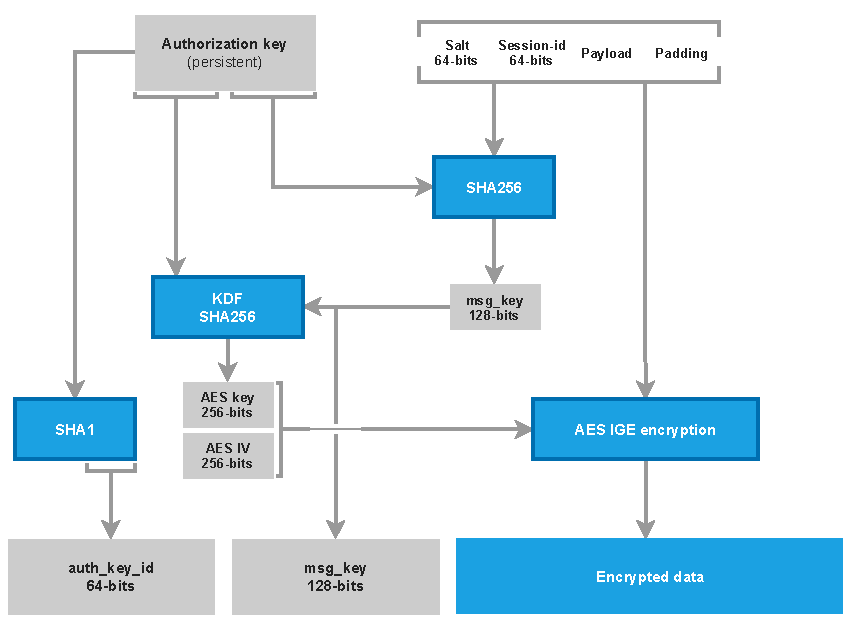
\includegraphics{cloud-chats}
    \caption{MTProto2.0 Cloud-chat protocol.\\Representation inspired by the Telegram official one.}
    \label{fig:cloud-chat-protocol}
    \end{figure}

Telegram uses the schema in \cref{fig:cloud-chat-protocol} to encrypt every message exchanged between the client and the server after an authorization key has been established using the authorization protocol in \cref{sec:auth-prot}.

A message key \textbf{msg\_key} of 128 bits is calculated as the middle 128 bits of the SHA256 of the entire message prepended by 32 bytes of the authorization key. The message itself contains a 64-bit salt, a 64-bit session id, the payload\footnote{The payload contains the time of the message, its length, a sequence number. Receiver should check these pieces of information, after decryption.} and a variable size padding of 12-1024 bytes.
The authorization key \textbf{auth\_key}, combined with the message key \textbf{msg\_key}, is used to derive a key and an initialization vector, which are used to encrypt the entire message using AES in IGE mode.

\subsection{IGE mode}
Infinite Garble Extension (in short, IGE) is a block cipher mode, lesser-known than others like ECB, CBC, OFB, CTR, CFB, GCM, CCM.
IGE can be defined with the following formula:

\begin{equation}
c_i = f_K(m_i \oplus c_{i-1}) \oplus m_{i-1}
\end{equation}

where $f_K$ stands for the encrypting function (like AES) with key $K$
and $i$ goes from 1 to $n$ $–$ the number of plaintext blocks. Two initialization vectors are also needed. \Cref{fig:IGE} summarizes how the encryption in IGE mode works.

\begin{figure}[t]
    \centering
    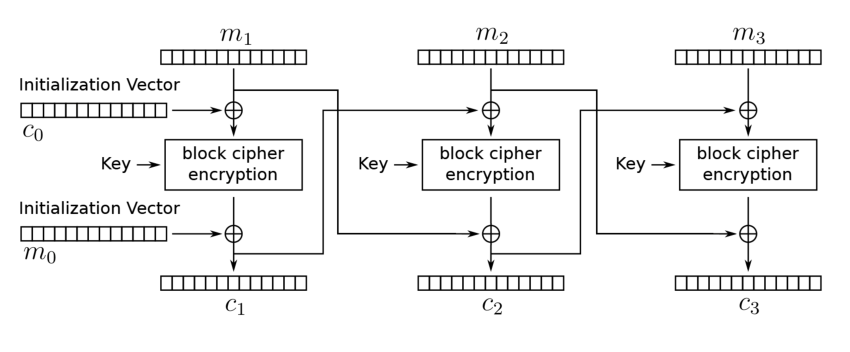
\includegraphics{IGE}
    \caption{Encryption in IGE mode.}
    \label{fig:IGE}
\end{figure}

One of the main properties of IGE mode is that it makes sure that if a ciphertext block is changed, then every subsequent block following it will not decrypt correctly.

As pointed out by \cite{Telegram-AFAQ-IGE}, the Telegram developers team is aware of the vulnerability of this mode to blockwise-adaptive Chosen Plaintext Attack (CPA)\cite{IGE-CPA}, but they claim that MTProto is not affected.




\section{Secret-chat protocol}
\label{sec:secret-chat}

%% Secret-chat protocol %%
\begin{figure}[!t]
\setlength{\instdist}{3cm}
\setmscoptions
\begin{msc}{}
\setmscscale{.8} 

\declinst{alice}{}{Alice}
\declinst{server}{}{Server}
\declinst{bob}{}{Bob}


\action*{\parbox{4.5cm}{\centering
    Knows $k_{AS}, k_{BS}$
}}{server}

\action*{\parbox{4.5cm}{\centering
    Knows $k_{AS}$
}}{alice}

\action*{\parbox{4.5cm}{\centering
    Knows $k_{BS}$
}}{bob}

\nextlevel[2]
\action*{\parbox{4.5cm}{\centering
    Gets $g, p$\\
    Generates $sid$\\
    $a \in \Z_p$\\
    $g_a := g^a \mod{p}$\\
    $M_1 := g, p, sid, g_a$
}}{alice}

\nextlevel[7]

%% TODO: Telegram webpage does not seem to specify HOW this is encrypted!!
%% UPDATE: It actually (kinda) does: it's encrypted as a cloud-chat message! For simplicity, keep this notation and explain its meaning in the written part.
\mess{$\left\{M_1\right\}_{k_{AS}}$}{alice}{server}
\nextlevel
\mess{$\left\{M_1\right\}_{k_{BS}}$}{server}{bob}

\nextlevel
\action*{\parbox{4.5cm}{\centering
    $b \in \Z_p$\\
    $g_b := g^b \mod{p}$\\
    $k_{AB} := g_a ^ b \mod{p}$\\
    $M_2 := sid, g_b, \mbox{fpk}\left(k_{AB}\right)$
}}{bob}

\nextlevel[6]
\mess{$\left\{M_2\right\}_{k_{BS}}$}{bob}{server}
\nextlevel
\mess{$\left\{M_2\right\}_{k_{AS}}$}{server}{alice}

\nextlevel
\action*{\parbox{5cm}{\centering
    $k_{AB} := g_b ^ a \mod{p}$\\
    Generates $payload$\\
    $mk := \mbox{sha256}\left(k_{AB}, payload\right)$\\
    $key, iv = \mbox{kdf}\left(k_{AB}, mk\right)$\\
    $C := \left\{payload\right\}_{key, iv}$
    $msg := \mbox{fpk}\left(k_{AB}\right), mk, C$
}}{alice}

\nextlevel[8]
\mess{$\left\{msg\right\}_{k_{AS}}$}{alice}{server}
\nextlevel
\mess{$\left\{msg\right\}_{k_{BS}}$}{server}{bob}

\end{msc}

\centering
\caption{MTProto2.0 Secret-chat protocol}
\label{fig:secret-chat-protocol}
\end{figure}

Telegram secret chats deal with end-to-end encryption between two clients (as usual, let us call the clients Alice and Bob, or A and B for brevity). After both clients have shared an authorization key with the Telegram server S, they can decide to engage themselves in a run of the secret chat protocol, allowing them to share, using a Diffie-Hellman key exchange, a shared secret. Notice that the server acts as a forwarder: every message sent from a client A to another client B is sent to the server, encrypted as a cloud chat message shown in \cref{sec:cloud-chat} with the authorization key of A; the server then decrypts the message and encrypts it as a cloud chat message using the authorization key of B and finally sends it to B. The writing $\left\{M\right\}_{k_{AS}}$ in \cref{fig:secret-chat-protocol} expresses that the message $M$ has been encrypted with the authorization key $k_{AS}$ using the cloud chat encryption schema.




\section{Rekeying protocol}
\label{sec:rekeying}

\chapter{Formalisation in Tamarin-Prover}

%% Fine dei capitoli normali, inizio dei capitoli-appendice (opzionali)
\appendix

% \chapter{Dolev-Yao model}
% \input{./chapters/app01_dolev_yao}

%% Parte conclusiva del documento; tipicamente per riassunto, bibliografia e/o indice analitico.
\backmatter

%% Riassunto (opzionale)
%\summary

%% Bibliografia (praticamente obbligatoria)
\bibliographystyle{plain_\languagename}%% Carica l'omonimo file .bst, dove \languagename � la lingua attiva.
%% Nel caso in cui si usi un file .bib (consigliato)
\bibliography{thud}
%% Nel caso di bibliografia manuale, usare l'environment thebibliography.

%% Per l'indice analitico, usare il pacchetto makeidx (o analogo).

\end{document}

--- Istruzioni per l'aggiunta di nuove lingue ---
Per ogni nuova lingua utilizzata aggiungere nel preambolo il seguente spezzone:
    \addto\captionsitalian{%
        \def\abstractname{Sommario}%
        \def\acknowledgementsname{Ringraziamenti}%
        \def\authorcontactsname{Contatti dell'autore}%
        \def\candidatename{Candidato}%
        \def\chairname{Direttore}%
        \def\conclusionsname{Conclusioni}%
        \def\cosupervisorname{Co-relatore}%
        \def\cosupervisorsname{Co-relatori}%
        \def\cyclename{Ciclo}%
        \def\datename{Anno accademico}%
        \def\indexname{Indice analitico}%
        \def\institutecontactsname{Contatti dell'Istituto}%
        \def\introductionname{Introduzione}%
        \def\prefacename{Prefazione}%
        \def\reviewername{Controrelatore}%
        \def\reviewersname{Controrelatori}%
        %% Anno accademico
        \def\shortdatename{A.A.}%
        \def\summaryname{Riassunto}%
        \def\supervisorname{Relatore}%
        \def\supervisorsname{Relatori}%
        \def\thesisname{Tesi di \expandafter\ifcase\csname thud@target\endcsname Laurea\or Laurea Magistrale\or Dottorato\fi}%
        \def\tutorname{Tutor aziendale%
        \def\tutorsname{Tutor aziendali}%
    }
sostituendo a "italian" (nella 1a riga) il nome della lingua e traducendo le varie voci.
